\documentclass[11pt,final,oneside]{fithesis}
\usepackage[utf8]{inputenc}
\usepackage[T1]{fontenc}
\usepackage{tipa}
\usepackage[slovak]{babel}
\usepackage{tabularx}
\usepackage{graphicx}
\usepackage{cite}
\usepackage{url}
\usepackage[nottoc]{tocbibind}

\hbadness=1000
\tolerance=1000

\newcommand{\smalltt}[1]{\small\texttt{#1}\normalsize}

\thesistitle{Monitorování zátěže a využití výpočetních zdrojů v heterogenním výpočetním prostředí}
\thesissubtitle{Diplomová práca}
\thesisstudent{Juraj Leždík}
\thesiswoman{false}
\thesisfaculty{fi}
\thesisyear{jar 2016}
\thesisadvisor{Mgr. Miroslav Ruda}
\thesislang{sk}
\begin{document}

\FrontMatter
\ThesisTitlePage

\begin{ThesisDeclaration}
\DeclarationText
\AdvisorName
\end{ThesisDeclaration}


\begin{ThesisThanks}
\end{ThesisThanks}

\begin{ThesisAbstract}
\end{ThesisAbstract}

\begin{ThesisKeyWords}
\end{ThesisKeyWords}

\tableofcontents
\addcontentsline{toc}{chapter}{Obsah}

\MainMatter
\chapter{Úvod}
Cloudová infraštruktúra MetaCentra poskytuje výpočetné prostriedky pre mnohé vedecké a výskumné organizácie. Spracovávajú sa v nej veľké objemy dát. Je tvorená mnohými uzlami rozmiestnenými naprieč celou
Českou republikou. Podstatou fungovania cloudového modelu je zdieľanie veľkého výpočetného výkonu viacerými subjektami, pre ktoré by zabezpečenie vlastnej infraštruktúry predstavovalo neúmernú 
ekonomickú, personálnu a prevádzkovú záťaž. Princípom zdieľania je, že prostriedky by mali byť ideálne využívané všetkými rovnako. Nemalo by dochádzať k tomu, že jeden klient vyťaží cloud natoľko, že 
výpočetné úlohy ostatných dostanú nepomerne malý priestor. To je možné docieliť monitorovaním využitia výpočtového výkonu a periférií. Ak máme informácie o tom, kto koľko využíval zdroje, je možné
tot využívanie účtovať a zároveň do budúcnosti primerane obmedzovať. 

Aby bolo možné správne vyvodzovať závery o zaťažení cloudu, je potrebné zberať údaje o tom periodicky a kontinuálne v čase. Je potrebné sledovať parametre v pravidelných intervaloch. Každému intervalu 
prináleží hodnota, ktorá vypovedá o využití prostriedkov v danom momente. Takéto dáta sa nazývajú časové rady. Cloud zahŕňa množstvo uzlov, kde na každom môže byť spustených množstvo úloh. O každej je
potrebné zberať viacero parametrov - vyťaženie procesora, pamäte, periférií. To predstavuje veľké množstvo metrických údajov, ktoré je potrebné ukladať a nejakým spôsobom vyhodnocovať. Slúžia na to 
databázy časových rád. Účtovanie sa tiež deje v určitých pravidelných intervaloch. Je preto potrebné mať možnosť spätne dohľadať údaje o využívaní zdrojov. Uchovávať podrobné metrické dáta má výnzam na určité
obdobie. Nie je potrebné vedieť ako bol využívaný cloud úlohou pred piatimi rokmi každých päť sekúnd. Okrem toho by to predstavovalo veľké požiadavky na úložné kapacity, ktoré by rástli lineárne vzhľadom
na počet úloh a čas. Je preto žiaduce po nejakej dobe dáta agregovať do väčších celkov a tiež mazať už nazbierané podrobné časové rady.

Aby boli monitorovacie údaje spoľahlivé, je potrebné zabezpečiť periodický zber metrických údajov. Monitorovanie sa uskutočňuje pravidelným pýtaním sa na vyťaženie daného zdroja. Aplikácia, ktorá zdroj
využíva, vytvorí odpoveď a pošle ju späť monitorovacej aplikácií. Problém nastáva, ak odpoveď nie je vytvorená v dostatočne krátkom intervale. Povedzme, že chcem zberať údaje každých päť sekúnd. Aplikácia,
ktorá práve rieši úlohy ale môže byť plne zaneprázdená a nebude odpovedať na výzvy na údaje o vyťaženosti. Tento problém je potrebné riešiť. Ak k tomu dôjde, nemali by byť vytvárané ďalšie výzvy na túto
zaneprázdnenú aplikáciu v takej miere, ako keď plynulo odpovedala. Monitorovacia aplikácia by si mala zapamätať poslednú nameranú hodnotu a tú odoslať ako aktuálnu. Zároveň by sa mala zaneprázdnenej aplikácií
pýtať v menej častých intervaloch. Ak aplikácia začne odpovedať, všetko je v poriadku. Ak nie, je možné reagovať reštartovaním monitorovacej aplikácie. Ak ani táto reakcia problém nevyrieši, komplikácia 
nastala zrejme v dotazovanej aplikácií.

Cloud predstavuje heterogénnu infraštruktúru. Na riešenie výpočetných úloh sa použivajú rôzne technológie a aplikácie. Rôzne aplikácie pristupujú k výpočetným problém odlišnými postupmi. Všetky úlohy 
sú ale počítané na akoby jednom veľkom a veľmi výkonnom počítači. Tieto aplikácie teda používajú spoločné zdroje. Metrické dáta, ktoré budem zberať, by takisto mali vypovedať o vyťažení tých istých druhov 
zdrojov. Je preto potrebné identifikovať, ktoré metrické dáta z jednej aplikácie je možné porovnať s údajmi z inej aplikácie. Takto môžeme dostať celkový obraz o tom, ako rôzne technológie využívajú
jednu skupinu zdrojov a len takto je možné vzájomne tieto technológie zrovnávať a účtovať ich využitie. 



\chapter{Cloudové technológie}
\section{Cloud}
Cloudové technológie umožňujú využívať veľkú množinu výkonných výpočetných zdrojov mnohým subjektom. Každý užívateľ cloudu využíva časť výpočetného výkonu. Spolu s rozdelením výkonu prichádzajú aj ďalšie výhody. Užívateľ sa nemusí starať
o podliehajúci hardvér. Typ fyzického procesora alebo rýchlosť pamäte uzla cloudu sú v určitom zmysle dôležité, ale pre výkon je rozhodujúca veľkosť pamäte, kapacita disku resp. počet procesorových jadier. Tieto požiadavky
cloud umožňuje jednoducho spravovať a transparentne meniť. Má to význam, ak sa rozrastú požiadavky užívateľa na výkon, alebo naopak z dôvodu obmedzenej prevádzky či 
nedostatku výpočetných úloh sa nároky môžu zmenšiť. Klient môže dané prostriedky využívať hneď, bez veľkých počiatočných investicií, ktoré by si buď nemohol dovoliť, alebo ak sú výpočetné úlohy krátkodonejšieho rázu, nákup
stroja s požadovaným výkonom by bol nevhodnou investíciou. Užívateľ sa nemusí starať o nákup hardvéru, jeho zostavovanie do funkčných serverov a ich následné rozširovanie a správu. Tieto služby zabezpečuje prevádzkovateľ cloudovej infraštruktúry.
Pre neho je zase dôležité mať prehľad o tom, ako sú jeho inštalované kapacity využívané. Či už z pohľadu skvalitňovania vlastných poskytovaných služieb alebo vo vzťahu ku klientovi a k tomu, v akej miere spotrebováva poskytovaný výkon.
Jednou z charakteristík cloudu je aj heterogénnosť v prístupe k zdrojom. Výpočetné prostriedky sú poskytované viacerými spôsobmi:

\begin{description}
\item[\emph{Infrastructure as a Service (IaaS)}] - Tento spôsob poskytuje užívateľovi priamo hardvérové prostriedky infraštruktúry. Ten má možnosť určiť, koľko pamäte, procesorov alebo diskovej kapacity požaduje. Je jeho voľbou
aký operačný systém použije, aký softvér nainštaluje a aké výpočetné úlohy bude realizovať alebo aké služby bude prevádzkovať.
\item[\emph{Platform as a Service (PaaS)}] - Užívateľ využíva priamo platformu prevádzkovateľa. Jedná sa vrstvu o úroveň vyššie ako pri využití infraštruktúry. Hardvérová konfigurácia je daná, ale užívateľ využíva operačný systém a 
súbor aplikácií na vývoj a prevádzku vlastných programov. Vlastník cloudu volí platformu a inštaláciu ďalšieho softvéru. Užívateľ ho môže používať a prípadne meniť. Tento spôsob poskytovania zdrojov znižuje záťaž na infraštruktúru
tak, že viacerí užívatelia využívajú jedno bežiace jadro operačného systému.
\item[\emph{Software as a Service (SaaS)}] - V cloudovej infraštruktúre môže byť nainštalovaný softvér, ktorý špecifickým spôsobom zefektívňuje prácu s distribuovanými výpočetnými zdrojmi. Je preto niekedy vhodné poskytovať samotné
prostredie jednej aplikácie ako službu. Užívateľ navrhuje výpočetné úlohy alebo aplikácie s využitím knižníc a architektúry konrétnej aplikácie a táto aplikácia sa zároveň stará o ich vykonávanie. 
\end{description}

Momentálne MetaCentrum poskytuje svoj dostupný výkon vo všetkých uvedeých formách. Jednotlivým prístupom zodpovedá konkrétne softvérové riešenie, ktorému sa budem venovať v jednej z nasledujúcich častí.

\subsection{Kontrola zdrojov cloudu}
Bez ohľadu na to, na akej vrstve si klient zvolí prístup k využívaniu zdieľaných výpočetných prostriedkov, jeho výpočty sa v konečnom dôsledku budú musieť realizovať na fyzickom hardvéri poskytovateľa. 
Aj keď sa daná úloha vypočítava na viacerých uzloch cloudu a rozličnými postupmi, vlastník by mal mať možnosť nejakým jednotným spôsobom určiť ako je reálne celá infraštruktúra vyťažovaná. K tomuto

\section{Virtuálne stroje}
Virtuálne stroje poskytujú úplnú virtualizáciu fyzickej hardvérovej štruktúry. Na jednom hosťujúcom počítači môže byť spustených viacero virtuálnych strojov. Každý má svoj vlastný virtuálny procesor, pamäť, grafický procesor, pevný disk 
a periférie. Operačný systém spustený vo virtuálnom stroji je izolovaný od hosťovského opračného systému (ak ho hosťovský počítač má). Takéto riešenie má jednu bezpečnostnú výhodu oproti aplikačným 
kontajnerom. Nežiadúce fungovanie jedného virtuálneho stroja neovplyvňuje beh ostatných.
V súčasnosti existuje mnoho úrovní virtuálnych strojov. Emulácia inštrukčnej sady, prekladanie programov za behu a ich optimalizácia, vysokoúrovňové virtuálne stroje (napr. Java) a systémové virtuálne stroje používané ako
jednotlivcami tak na serveroch.

\subsection{Hypervízor}
Hypervízor je softvér, ktorý vytvára a zabezpečuje beh virtuálnych strojov. Rozlišujeme 2 typy:
\begin{description}
\item[natívny] - na hosťujúcom počítači nie je nainštalovaný žiadny operačný systém. Hypervízor spravuje hardvér hosťujúceho počítača a kontroluje beh operačných systémov, ktoré sa javia ako procesy.
Príkladom je VMware ESX/ESXi, Oracle VM Server for x86 alebo Citrix XenServer.
\item[hosťovaný] - hypervízor je spustený ako bežný program v operačnom systéme hosťujúceho počítača. Príkladom je QEMU, VMware Workstation alebo VirtualBox.
\end{description}
\cite{hypervisorTypes}

\section{Aplikačné kontajnery}
Kontajnery predstavujú odlišný prístup k virtualizácií ako virtuálne stroje. Tiež ide o snahu spúšťať softvér v prostredí oddelenom od skutočného hardvéru a operačného systému. Na rozdiel od úplných virtuálnych strojov 
nie je virtualizovaný celý hardvér, ale len softvérové vybavenie nevyhnutné na spustenie programu. Rozdiel v architektúre ilustruje nasledovný obrázok: 
\begin{figure}[h]
\begin{center}
       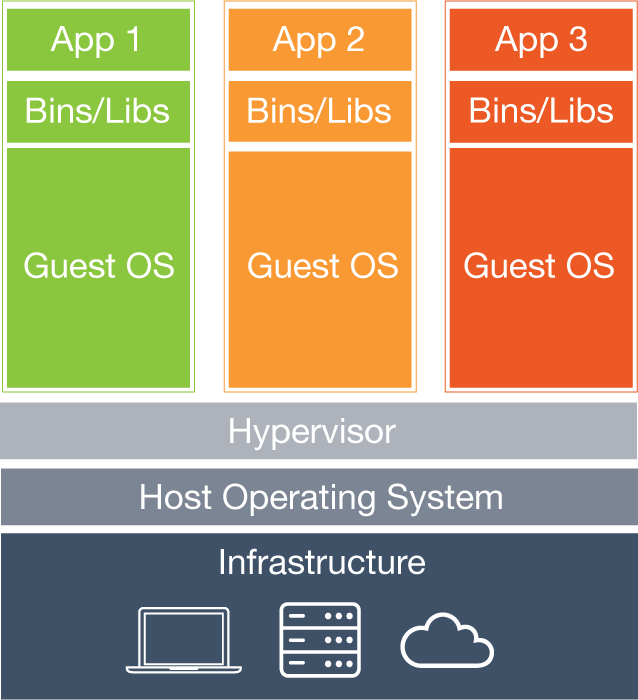
\includegraphics[width=0.8\textwidth]{images/docker.png}
       \caption{Porovnanie architektúry Docker a virtuálnych strojov}\cite{docker}
\end{center}
\end{figure}
V kontajneri môže byť spustený nezávislý operačný systém spolu s požadovanými aplikáciami. Hosťovský počítač, na ktorom sú kontajnery spustené, má jeden operačný systém a jednu množinu prostriedkov, 
ktoré tieto kontajnery zdieľajú. Jednotlivé kontajnery dostávajú kontrolovaný prístup k výpočtovému výkonu, pamäti, úložnej kapacite, sieti a prípadne ďalším prostriedkom.




\section{MapReduce aplikačné prostredia}



\section{Cloudové technológie MetaCentra}
\subsection{libvirt/KVM}
KVM\footnotemark\footnotetext{Kernel-based Virtual Machine} je plné virtualizačné riešenie pre Linux pre x86 hardvér, obsahujúce virtualizačné rozšírenia (Intel VT or AMD-V).
Pozostáva z nahrateľného modulu jadra, kvm.ko, ktorý poskytuje základ virtualizačnej infraštruktúry a šepcifický modul, kvm-intel.ko alebo kvm-amd.ko. Je možné virtualizovať obrazy 
s operačným systémami Linux aj Windows. Každý virtuálny stroj má vlastný virtualizovaný hardvér: sieťovú kartu, disk, grafický adaptér, atď. KVM je open-source softvér. Virtualizačný modul jadra
sa nachádza v Linuxe od verzie 2.6.20.\cite{kvm}

libvirt je sada nástrojov na prácu s virtualizačnými schopnosťami Linuxu (a ostatných OS). Je to voľný softvér dostupný pod licenciou GNU LGPL. 
Obsahuje API v jazyku C a väzby pre bežné programovacie jazyky.\cite{libvirt}

\subsection{Docker}
Docker umožňuje zabaliť aplikáciu so všetkými jej závislosťami do štandardizovanej jednotky (tzv. kontajnery) určenej na softvérový vývoj. Kontajnery Dockeru obaľujú softvér kompletným súborovým systémom, ktorý
zahŕňa všetko, čo daný softvér potrebuje na spustenie: kód, nástroje potrebné na beh, systémové nástroje a knižnice. Toto zaručuje, že program bude pracovať rovnako bez ohľadu na prostredie, v ktorom
je spustený.\cite{docker}


\subsection{Hadoop}
Projekt Apache Hadoop vyvíja open-source softvér na spoľahlivé, škálovateľné, distribuované výpočty. Apache Hadoop je prostredie, ktoré umožňuje distribuované spracovávanie veľkých množstiev dát
naprieč clustermi, používajúcimi jednoduché programovacie modely. Je navrhnutý tak, aby bol škálovateľný od jednotlivých serverov po tisícky strojov, kde každý poskytuje lokálny výpočetný výkon a úložný priestor.
Nespolieha sa na vysokú dosupnosť hardvérových prostriedkov, ale je navrhnutý, aby detekoval a zvládal chyby na aplikačnej vrstve, takže poskytuje vysoko dostupnú službu nad clusterom počítačov, 
z ktorých každý je náchylný na chyby.

Projekt pozostáva z týchto modulov:
\begin{description}
\item[\emph{Hadoop Common:}] spoločné nástroje, ktoré podporujú ostatné Hadoop moduly
\item[\emph{Hadoop Distributed File System (HDFS™):}] distribuovaný súborový systém, ktorý poskytuje vysokú priepustnosť
\item[\emph{Hadoop YARN:}] prostredie pre plánovanie úloh a správu zdrojov clustera
\item[\emph{Hadoop MapReduce:}] systém založený na YARN pre paralelné spracovávanie veľkých množstiev dát, prostredie pre plánovanie úloh a správu zdrojov clustera
\end{description}


\chapter{Zber a uchovávanie monitorovacích dát}
Monitorovanie akejkoľvek (nielen počítačovej) prevádzky je dôležitá oblasť, ktorá má význam pre jej správne fungovanie a jej správu, zdokonaľovanie a servis. Na priblíženie uvediem príklad železničnej spoločnosti. 
Je vhodné vedieť, koľko ľudí prepraví spoločnosť na určitom spoji. Tak môže identifikovať nerentabilné spoje, prípadne spoje, ktoré sú preťažené
a je potrebné nejakým spôsobom zväčšiť ich kapacitu. Iným príkladom môže počet vlakov, ktoré prejdú za deň jednou stanicou. Vo všeobecnosti sa teda jedná o vyťaženie zdrojov vlakovej spoločnosti, či už sú to samotné
vlaky alebo stanice, prípadne personál atď. Monitorovanie nám poskytuje dáta, ktoré majú viacero aplikácií:
\begin{description}
\item[\emph{Prehľad o aktuálnom vyťažení zdrojov}]
Pri zbere dát toto zodpovedá meraniu konkrétnej hodnoty sledovaného parametru. Kvantifikáciou sledovaného zdroja dostaneme predstavu o tom, ako je používaný "teraz", čiže v prítomnosti. Môžeme tak detegovať prípadné
preťaženie zdroja, jeho dostupnosť alebo zlyhanie.
\item[\emph{Prehľad o vyťažení zdrojov za určitú dobu}]
Vyťaženie zdrojov sa v priebehu času mení. Nielen z krátkodobého hľadiska, kedy napríklad viac ľudí cestuje ráno za prácou a do školy, ale aj zo strednodobého (v období leta ľudia viac cestujú na dovolenky, čiže sa menia 
vyťažené spoj) a dlhodobého hľadiska (cestujúcich stále pribúda). Uchovávanie monitorovacích dát predstavuje kľúčový požiadavok, aby sme mohli sledovať, aké trendy vo využívaní mali jednotlivé sledované zdroje v priebehu nejakej doby.
Z takto nahromadených dát môžeme vypočítavať rôzne štatistiky a ďalej ich analyzovať.
\item[\emph{Prehľad o vyťažení zdrojov podľa parametrov}]
Vyťaženie konkrétneho vlaku môže predstavovať jednoduché čislo, ktoré reprezentuje, koľko ľudí sa nachádzalo vo vlaku. Spoločnosť ale prevádzkuje viacero druhov vlakov a množstvo liniek na rôznych. Chceme preto mať možnosť
zistiť napr. tom, ako bol využívaný rýchlik na trati Brno-Břeclav cez prázdniny v utorky ráno. Okrem jednoduchého tvrdenia, že vo vlaku bol nejaký počet cestujúcich, nám dobre nastavené monitorovanie poskytuje aj komplexnejšie
informácie.
\item[\emph{Prehľad o stave zdrojov z hľadiska správy a plánovania}]
Nezanedbateľný význam má monitorovanie z hľadiska údržby a servisu poskytovaných služieb. Z dostupných dát vieme indentifikovať nefunkčný zdroj a nahradiť ho novým. V prípade vysokého vyťaženie zas môžeme vyvodiť záver, že zdroje už nie sú
dostačujúce a je potrebné ich nejakým spôsobom rozšíriť prípadne zlepšiť efektivitu ich využívania. Takisto vieme do určitej miery predpovedať, ako budú zdroje v budúcnosti využívané, čo je podstatné pri samotnom plánovaní 
odstávok, servisnej činnosti alebo dočasného rozšírenia zdrojov.
\item[\emph{Účtovanie vyťaženia zdrojov}]
Každá poskytovaná služba má svojho spotrebiteľa. Či už sa jedná o zákazníkov železničnej spoločnosti alebo klientov výpočetného strediska. Dáta o používaní zdrojov sú jediným možným spôsobom ako rozumne stanoviť cenu za používané zdroje.
Taktiež na ich základe môžeme sledovať činnosť jednotlivých užívateľov v systémoch a stanoviť im akceptovateľné podmienky na využívanie služieb.
\end{description}

\section{Všeobecné problémy monitorovania}
Problematika monitorovania v sebe zahŕňa viacero aspektov, ktoré možno oddeliť, zistiť pre ne najlepšie riešenia a spojiť ich tak do funkčného celku. 
\\
\\ \emph{Identifikácia relevantných metrík}
\\
V prvom rade je potrebné identifikovať, čo vlastne potrebujeme pre konkrétny systém
monitorovať. Jedná sa o určenie zdrojov kľúčových pre dané prostredie. Pre železničnú spoločnosť to môže byť vyťaženie vlakov alebo množstvo spotrebovanej energie. Niektoré údaje, ktoré potrebujeme vedieť, je možné odvodiť z iných už
nameraných hodnôt. Takéto meriky budem nazývať sekundárne. Nakoľko môžu byť dopočítané, nie je vždy nevyhnutné ich v čase sledovať a uchovávať.
\\
\\ \emph{Analýza v reálnom čase a varovania}
\\
\\Namerané hodnoty metrík je okrem neskoršej štatistickej analýzy potrebné sledovať a analyzovať v reálnom čase. Metrika môže mať svoje kritické hodnoty. Sú to hodnoty, ktoré naznačujú, že daný zdroj sa vymyká bežným očakávaniam o využití.
Na toto je vhodné reagovať. Či už sa jedná o zapísanie hlásenia do logu, zobrazenie varovania alebo prípadné zaslanie emailu či sms správy s popisom udalosti.
\\
\\ \emph{Meracie intervaly}
\\
Ďalším čiastkovým problémom je granularita metrík. Zdroje sú kontinuálne využívané v čase. Tieto dáta je potrebné nejakým spôsobom digitalizovať. V určitom momente sa pozrieme na zdroj, kvanitifikujeme, do akej miery je využitý a danú
hodnotu zobrazíme prípadne uložíme. Meranie je po uplynutí určitého intervalu zopakovať, aby sme získali opäť aktuálne údaje. Rôzne zdroje sa menia v čase rôznou intenzitou. Napr. kapacita vlaku sa v priebehu jazdy mení zriedkavo, zatiaľčo
počet cestujúcich sa mení v každej stanici. Je preto dôležité určiť aj periodicitu zberania jednotlivých metrík. Niektoré metriky sa môžu meniť takým spôsobom, že nie je efektívne sledovať ich zmenu pravidelne v nejakých intervaloch. Namiesto
toho je efektívnejšie pri zmene daného parametru túto zmenu ohlásiť spolu s novou hodnotou. U vlakov je to napríklad kapacita vlaku, ktorá sa mení len zriedkavo počas jazdy, napríklad pri prepriahaní vozňov z jedného vlaku do druhého.
\\
\\ \emph{Počet zdrojov}
\\
Množstvo zdrojov predstavuje ďalšiu oblasť, ktorú je potrebné zvážiť. Môžeme disponovať rôznym počtom zdrojov viacerých druhov, rozmiestnenými na viacerých miestach pod správou mnohých ľudí - prípadne oddelení. Metrické dáta vo svojej
podstate len kvantifikujú využitie zdroja vo všeobecnosti. Zaobchádzajú s ním v tom zmysle, ako by bol len jeden. Napr. metrika vyťaženie vlaku v počte osôb. Nehovoria nič bližšie o tom, o aký zdroj sa jedná, kde je ho možné nájsť. V rámci širšieho
systému je preto dôležitá jednoznačná identifikácia daného zdroja. O danom vlakom preto chceme zistiť napr. jeho názov, linku na ktorej premáva a prípadné ďalšie technické údaje. Takéto údaje sa nazývajú metadáta - čiže dáta o (v tomto 
prípade o metrických) dátach.
\\
\\ \emph{Ukladanie dát}
\\
Uchovávanie metrických dát je kľúčovou sučasťou monitorovacieho systému. Doba, po ktorú vlastníci zdrojov uchovávajú metrické dáta, sa líši systém od systému. V niektorých oblastiach to je dokonca upravené zákonmi - napr. telekomunikácie,
v iných je to na zvážení majiteľa ifraštruktúry. Množstvo dát, ktoré je treba uložiť, závisí od viacerých parametrov. Sú nimi počet druhov zdrojov, počet jednotlivých inštancií zdrojov, počet metrík, ktoré sa o zdrojoch
uchovávajú, periodicita zbieraných metrík a do určitej miery aj spôsob identifikácie daného zdroja. Prikladám tabuľku, ktorá ilustruje ako sa mení počet záznamov v závislosti na uvedených parametroch.
\\Ukladanie metrických dát predstavuje zároveň úzke hrdlo monitorovacieho riešenia. Zistenie hodnôt metrík pre kontrétny zdroj predstavuje v zásade serializovanú činnosť. V určitom čase sú všetky zdroje opýtané na to, ako sú vyťažené. Po jednom
zistia svoje hodnoty a odošlú ich na uloženie. Počet metrík pre jeden zdroj je v bežnej praxi len zlomkom počtu zdrojov. Na časť systému, ktorá je zodpovedná za ukladanie metrík, sú preto v pravidelných intervaloch kladené pomerne 
veľké nároky. Je ich už ale možné spracovávať paralelne. Centralizácia úložiska by znamenala prílišnú záťaž a monitorovacie uzly, preto je vhodné, aby takéto úložisko bolo distribuované a prispôsobené na paralelné spracovávanie veľkých
objemov dát.
\\
\\ \emph{Vizualizácia a analýza dát}
\\
Zozbierané metrické dáta je ďalej potrebné nejakým spôsobom zobraziť. Na to sú vhodné čiarové grafy s dvoma osami, kde horizontálna os predstavuje čas a vertikálna os predstavuje hodnotu nameranej metriky.
Analýza zozbieraných dát slúži na odhalenie trendov vo využívaní zdrojov a môže viesť k zdokonaľovaniu systému a k lepšiemu plánovaniu využívania zdrojov.


\subsection{Monitorovanie v heterogénnom výpočetnom prostredí}
V oblasti cloudového a gridového výpočetného prostredia je pre monitorovanie kľúčové sledovať vyťaženie výpočetných zdrojov. Konkrétne procesor, výpočetná pamäť, trvalý ukladací priestor a sieťová infraštruktúra. Toto je spoločné
pre všetky technológie a okrem týchto zdrojov je vhodné sledovať aj parametre špecifické pre jednotlivé oblasti. Tým sa budem konkrétne venovať v kapitole Metriky.
\\Automatizované monitorovanie výpočetného prostredia so sebou prináša aj špecifické problémy. Odvíjajú sa od toho, že monitorovanie je vykonávané strojovo (tj. pomocou počítača) a monitorované zdroje sú takisto stroje, ktorých
stav z pohľadu využitia sa mení veľmi dynamicky.
\\Rozdielny je aj prístup jednotlivých technológií v tom, ako poskytujú výpočetné zdroje. Aplikačné kontajnery a virtuálne stroje sa snažia rozdeliť celú infraštruktúru na menšie viac-menej uzavreté celky, ktoré sú potom sprostredkované
užívateľom. Každý tento celok má pridelené zdroje, ktoré potom využíva. Množstvo týchto zdrojov je možné meniť, ale súvisí to s reštartovaním virtuálneho stroja alebo kontajnera. Z pohľadu gridu sú zanedbávané zdroje jedného uzla a na
vypočítavanie úloh sa berú do úvahy všetky zdroje celého clustera. 

\subsubsection{\textbf{Problematika intervalov}}
U vysoko výkonných výpočetných systémov sa jednotlivé operácie vykonávajú vo veľmi krátkych časových intervaloch. Rádovo sú to nanosekundy. Jednotlivé procesy a výpočetné úlohy dostávajú na krátky čas k dispozícií všetky zdroje, čím 
sa z vyššieho pohľadu zabezpečuje paralelizácia. To spôsobuje vyťaženie množstva inštancií zdrojov mnohými učastníkmi. Celkový stav infraštruktúry z pohľadu vykonaných úloh a prenesených dát sa preto mení veľmi dynamicky a je vhodné
zbierať dáta o zdrojoch v rozmedzí jednej až troch sekúnd. 
\\Nezanedbateľnú rolu hrá aj čas potrebný na získanie jedného takéhoto "snímku" využitia zdrojov. Kým v prípade vlakov je napr. dostatok času na spočítanie cestujúcich medzi jednotlivými zastávkami, v prípade heterogénneho prostredia 
môže byť tento čas kritický. Ak sa každé dve sekundy pýtame na metrické údaje, očakávame, že odpoveď príde v kratšom intervale. V najlepšom prípade by táto doba odpovede mala byť len malý zlomok periódy danej metriky. Vopred nevieme,
koľko bude trvať, kým príde odpoveď. To je v priamej závislosti od toho, koľko subjektov infraštruktúru využíva a koľko úloh spúšťa. Ak je však doba odpovede dlhšia ako samotný interval metriky, je to potrebné nejako riešiť. Nie je 
vhodné automaticky paralelne vygenerovať ďalšiu požiadavku na "snímku". Žiaducejším spôsobom riadenia je také, ktoré počká, kým sa daná požiadavka vykoná, a potom v nasledovnom intervale je meranie vykonané znova. Týmto sa predíde nadmernej záťaži
celého systému.
\\To, ako sa systém vysporiadava z takýmto neočakávaným správaním, som zohľadňoval pri jednotlivých dostupných softvérových riešeniach.

\subsubsection{\textbf{Detekcia nových zdrojov a užívateľov}}
Heterogénna štruktúra v čase mení aj množstvo a kapacitu svojich poskytovaných zdrojov. Nie je možné staticky definovať zoznam procesorov, diskov, alebo virtuálnych strojov ktoré treba monitorovať. Podobne je to aj s užívateľmi. Proces
vytvárania nových užívateľov je zautomatizovaný, takisto užívatelia môžu automatizovať vykonávanie svojich výpočetných úloh. Monitorovacie riešenie sa preto musí vedieť vysporiadať s týmito dynamickými zmenami, musí ich vedieť 
automaticky detegovať a zberať o nich metrické dáta.

\section{Časové rady}
Monitorovacie dáta vo svojej podstate predstavujú časové rady.
Časová rada je sekvencia dát, kde danému časovému okamihu zodpovedá jedna hodnota. Príkladom je zaznamenávanie teplôt v priebehu roka, výšky oceánskeho prílivu alebo množstvo áut, ktoré za určitú dobu
prejde jedným bodom diaľnice. Efektívnou metódou vizuálizácie dát časových rád sú čiarové grafy. Horizontálna os reprezentuje plynutie času a na vertikálnej osi sú znázornené hodnoty v danom čase.

\subsection{Analýza časových rád}
Analýza časových rád sa primárne zaoberá získavaniu štatistík o zozbieraných dátach, napr. priemerná teplota počas celého roka. Medzi ďaľšie úlohy patrí:
\begin{description}
\item[\emph{Exploračná analýza dát}]
\item[\emph{Aproximácia na funkciu}] 
\item[\emph{Predpovedanie}] 
\item[\emph{Klasifikácia}] 
\end{description}
Mám sa viac o nich rozpísať?

\subsection{Zaobchádzanie s historickými dátami}
Niečo o tom, ako sa v rámci šetrenia priestoru dáta zhlukjú a vypočítavajú sa agregované štatistiky.

\chapter{Aktuálne monitorovacie riešenia}
Problematike monitorovania softvéru a infraštruktúry sa venuje viacero komerčných alebo open-source aplikácií, prípadne aplikácií zadarmo. Rôznymi technológiami riešia zber dát, ich uchovávanie, vizualizáciu a operácie nad
nimi. Najprv sa venujem popisu aplikácií, ktoré súvisia so samotným monitorovaním dát, neskôr rozoberám dostupné riešenia v oblasti uchovávania časových rád.

\section{Linux cgroups}
Linux cgroups je technológia linuxového jadra, ktorá umožňuje limitovať, sledovať a izolovať spotrebu prostriedkov systému jednotlivými procesmi. Zavádza stromovo organizované kontrolné skupiny. 
Kontrolná skupina obsahuje obmedzenia pre jeden systémový prostriedok, tzv. susbsystém. Príklad subsystémov, ktoré poskytuje Red Hat Enterprise Linux: 
\begin{description}
\item[\emph{blkio}] - this subsystem sets limits on input/output access to and from block devices such as physical drives (disk, solid state, USB, etc.).
\item[\emph{cpu}] - this subsystem uses the scheduler to provide cgroup tasks access to the CPU.
\item[\emph{cpuacct}] - this subsystem generates automatic reports on CPU resources used by tasks in a cgroup.
\item[\emph{cpuset}] - this subsystem assigns individual CPUs (on a multicore system) and memory nodes to tasks in a cgroup.
\item[\emph{devices}] - his subsystem allows or denies access to devices by tasks in a cgroup.
\item[\emph{freezer}] - this subsystem suspends or resumes tasks in a cgroup.
\item[\emph{memory}] - this subsystem sets limits on memory use by tasks in a cgroup, and generates automatic reports on memory resources used by those tasks.
\item[\emph{net\_cls}] - this subsystem tags network packets with a class identifier (classid) that allows the Linux traffic controller (tc) to identify packets originating from a particular cgroup task.
\item[\emph{net\_prio}] - this subsystem provides a way to dynamically set the priority of network traffic per network interface.
\item[\emph{ns}] - the namespace subsystem.
\end{description}

Pre každý subsystém existuje jeden strom kontrolných skupín. Ďalej skupina obsahuje zoznam procesov, ktoré podliehajú definovaným obmedzeniam. V strome kontrolných skupín sa proces vyskystuje len raz.
V cloudovom prostredí však jednotlivé technológie využívajú a spúšťajú mnoho procesov, ktoré by sa obtiažne priraďovalo jednotlivým užívateľom v súvislosti so spustenými aplikáciami, preto tento spôsob
monitorovania nie je úplne vhodný. Takisto zberané metriky o subsystémoch sú agregované pre kontrolnú skupinu, tj. predstavujú súčet pre skupinu procesov, takže nie je možné jednoznačne určiť koľko zdrojov spotreboval
ten ktorý proces.

\section{Nagios}
Nagios je aplikácia, ktorá poskytuje komplexné riešenie na monitorovanie systémov. Poskytuje informácie o kľúčových komponentoch infraštruktúry vrátane aplikácií, služieb, operačného systému, sieťových protokolov, systémových metrík
a sieťovej infraštruktúry. \cite{19} Aplikácia pozostáva z jadra, ktoré riadi zber údajov, a z množstva pluginov tretích strán. Tie sa zaoberajú monitorovaním jednotlivých oblastí systému. Ďalej aplikácia
poskytuje grafické užívateľské rozhranie v podobe webového rozhrania. K dispozícií sú rôzne vizualizácie nameraných dát, grafy a histogramy. Nagios disponuje aj systémom užívateľských účtov. Tie sa delia na dva typy: 
administrátorov a bežných užívatešov. Bežní užívatelia majú prístup k nameraným hodnotám a zobrazovaniu grafov. Administrátori môžu konfigurovať aplikáciu, pridávať služby, ktoré je potrebné monitorovať,
 upravovať parametre monitorovania a spravovať užívateľské účty. K dispozícií je aj uchovávanie konfigurácie aplikácie a spravovanie týchto konfigurácií. Súčasťou je aj systém na upozorňovanie na kritické
 hodnoty, či už formou emailu alebo SMS správou. Aplikácia je vyvíjaná pre platformu CentOS a Red Hat Enterprise Linux. Namerané metriky sa uchovávajú v logovacích súboroch. 
 Pomocou pluginov je možné ich odosielať do MySQL databázy prípadne PostgreSQL. Nagios predstavuje centralizované riešenie pre  monitorovanie, kde výkonné jadro riadi zberanie metrík naprieč celým systémom. 
 Jadro a pluginy sú dostupné zdarma, komplexné riešenie je potrebné zakúpiť. Cena sa odvíja od množstva zariadení, ktoré je potrebné monitorovať. Zariadením sa rozumie niečo, čo má IP adresu, 
 prípadne doménové meno - či už sa jedná o firewall, switch, router, pracovnú stanicu alebo server. V súčasnosti Nagios disponuje pluginmi Docker, Hadoop aj libvirt/KVM, no ani jeden z pluginov 
 nemonitoruje požadované metriky.

\subsection{PluginAPI}
Nagios pluginy existujú vo forme skriptov alebo spustiteľných programov. Aby mohli fungovať ako pluginy ich činnosť musí spĺnať dve kritériá. Prvým je výpis aspoň jedného riadku na štandardný výstup.
Ten sa týka nameraných metrík. Od verzie 3 je podporovaných aj viacerov riadkov na výstupe. Druhým kritériom je návratová hodnota.
API rozoznáva štyri návratové hodnoty. Tie zodpovedajú stavom monitorovanej služby - či je služba v poriadku, či vygenerovala nejaké varovanie, či je jej stav kritický, alebo neznámy. Prednastavená maximálna dĺžka 
výstupu je 4 kB, je ju však možé pomocou konfigurácie zmeniť.

\subsection{Riadenie intervalov zberu metrík}
Pre jednotlivé monitorovacie sondy je možné nadefinovať interval v počte sekúnd, v ktorom je potrebné aby sonda ukončila svoju činnosť. Ak sa tak nestane, proces sondy je ukončený a jej návratová hodnota
zaznamenaná ako kritická. Taktiež je toto zaznamenané do logov Nagiosu. Tento mechanizmus predstavuje akúsi poslednú záchranu pred zahltením systému pluginmi, ktoré sa nesprávajú podľa očakávaní.

\section{Zabbix}
Zabbix je open-source aplikácia na monitorovanie systémov od malých systémov s malým počtom uzlov až po veľké firemné prostredia s tisíckami strojov. Architektúra aplikácie pozostáva zo serveru a agentov.
Úlohou agentov je zber monitorovacích dát a ich odosielanie serveru. Komunikácia týchto dvoch častí môže prebiehať dvoma spôsobmi. V prvom prípade si agent vyžiada zoznam metrík, ktoré má sledovať. Následne 
serveru odosiela všetky tieto metriky po jednom. Druhou alternatívou je postup, kedy sa server agenta pýta na jednotlivé hodnoty metrík a ten mu ich odosiela. Server spravuje konfiguráciu jednotlivých agentov,
čo uľahčuje ovládanie ich správania naprieč celou infraštruktúrou.
\\Aplikácia zberá udáje o dostupných zdrojoch uzlov, o počte procesorov, dostupnej pamäti a úložnej kapacite. Taktiež zberá údaje o aktuálnom vyťažení týchto zdrojov. Okrem toho sleduje dostupnosť a parametre
služieb ako FTP, DNS, HTTP, SMTP, SSH a rôznych ďalších. Taktiež poskytuje údaje o proces bežiacich v systéme a o užívateľoch. Zaujímavým prvkom je monitorovanie logov, ich analýza a vytváranie varovaní 
v prípade, že je to nutné.
\\Zabbix vie zberané dáta vizualizovať pomocou grafov. Súčasťou je aj sledovanie zberaných hodnôt, ich kontrola na požadovaný rozsah a generovanie notifikácií. Poskytuje aj manažment užívateľov samotnej 
aplikácie a ich práv na zaobchádzanie s ňou. Zabbix podporuje autodetekciou nových prvkov v infraštruktúre. Kontroluje zadaný sieťový rozsah na nové uzly, služby na nich bežiace alebo automaticky registruje
nových spustených agentov.
\\Na zvládanie záťaže vo veľkých systémoch je zavedený systém proxy serverov. Tie zhlukujú dáta z niekoľkých agentov a až potom sú odosielané centrálnemu serveru.
\\Zabbix má vlastnú databázu na uchovávanie zozbieraných dát. Rozdeluje ich na históriu a trendy. História sú dáta tak, ako boli namerané, trendy predstavujú agregované dáta z pohľadu dlhších období, napr. v 
rádoch rokov.
\\V súčasnosti Zabbix nepodporuje zber metrík z Hadoopu. Je možné nainštalovať agenta do kontajneru alebo virtuálneho stroja. To ale nepredstavuje ideálne riešenie, nakoľko tieto služby v prvom rade
slúžia pre potreby užívateľov a je chodné nechať na nich, čo v danom kontajneri alebo virtuálnom stroji chcú mať spustené.

\subsection{Riadenie intervalov zberu metrík}
Konrola zberu jednotlivých metrík z hľadiska doby trvania tohoto zberu sa v Zabbixe odohráva na úrovni agenta a serveru. Na úrovni agenta ide o čas, ktorý je možné stráviť spracovávaním a získavaním
jednotlivých metrík. Pre server je potom definovaná doba, ktorú je ochotný čakať na odpoveď agenta. Tieto doby je možné konfigurovať v rozsahu od 1 do 30 sekúnd.
\cite{20}
\cite{05}
Zabbix nespracuje jednoduchú kontrolu na hodnotu metriky, ktorá trvá dlhšie ako túto dobu.
\cite{04}
Dokumentácia však neuvádza, ako sa aplikácia riadi beh externých procesov, ktoré zberajú dáta.

\subsection{Moduly}
Aplikáciu je možné rozšíriť o vlastné moduly zberajúce dáta tromi spôsobmi. \cite{06}
\begin{description}
\item[\emph{užívateľské parametre}] - v tomto prípade užívateľ definuje v agentovi názov metriky a príkaz, ktorý sa má vykonať na zber jej hodnoty
\item[\emph{externé kontroly}] - jedná sa o kontrolu na strane servera, kedy je tiež definovaný skript zberajúci dáta a server ho spúšťa
\item[\emph{system.run}] - jedná sa o kontrolu na strane agenta, ktorá podporuje väčší výstup spusteného príkazu ako len hodnota metriky
\end{description}
Okrem toho poskytuje aj programové API a vývoj vlastných modulov ako zdieľaných knižníc, ktoré musia implementovať požadované funkcie.

\section{Icinga}
Icinga predstavuje open-source monitorovací nástroj, ktorý je nástupcom Nagiosu. Je založená na princípe paralelnej činnosti viacerých vlákien, čo poskytuje možnosť vykonávať množstvo meraní
za krátky časový interval. Zabezpečuje monitorovanie záťaže zdrojov ako disk, CPU, pamäť a sieť a to v operačných systémoch na základe Linuxu a aj v prostredí Windows. Ďalej podporuje zberanie
dát o mnohých ďalších službách, ako je monitoring databáz, odozvy serverov, webových služieb, výkonu JVM, sledovanie logov. Podporuje monitorovanie virtualizačnej platformy VMWare. 
Poskytuje aj bežné mechanizmy v oblasti monitorovania ako generovanie notifikácií o neštandardnom správaní, na ktoré je možné reagovať spustením nejakého systémové príkazu. Na ukladanie dát 
používa svoju databázu, no podporuje aj odosielanie dát do databázy časových rád InfluxDB.
\\V súčasnosti Icniga nie je schopná monitorovať ani jednu zo služieb v prostredí MetaCentra.

\subsection{Rozšíriteľnosť aplikácie}
Icinga poskytuje systém, akým je možné do nej pridať kontroly nových metrík, prostredníctvom tzv. check príkazov. Jedná sa o kofiguračné objekty, kde užívateľ definuje príkaz,
ktorý sa má spustiť, spolu s hodnotami jeho argumentov. Icinga určí stav tejto kontroly podľa návratovej hodnoty príkazu.\cite{08} Hodnoty a názvy metrík sú vracané vo forme textového výstupu.

\section{collectd}
Collectd je open-source monitorovacia aplikácia vyvinutá v jazyku C. Má architektúru jadra a pluginov, ktoré sa starajú o mnoho činností súvisiacich s monitorovaním od zbierania dát, cez
zapisovanie metrík a sledovanie prahových hodnôt a upozorňovanie. Jadro predovšetkým ovláda a kontroluje vykonávanie týchto aktivít. V pravidelných intervaloch spúšťa kontroly metrík, 
analyzuje namerané hodnoty, generuje notifikácie v prípade, že hodnoty sú mimo požadovaný rozsah, alebo ak nedorazili 
v požadovaných intervaloch. V súčasnosti je k dispozícií viac než 90 pluginov. Poskytujú monitorovanie základných výpočetných zdrojov ako sú procesor, pamäť, disky a sieťové rozhrania, ďalej monitorovanie
mnohých aplikácií (napr. databázy, e-mail, webové servery) a protokolov. Zvolený programovací jazyk dáva dobré predpoklady na výkon a prenositeľnosť, čo umožňuje beh na systémoch bez 
skriptovacích jazykoc alebo cron démona, ako napríklad zabudované systémy. Zároveň ale disponuje optimalizáciami a prvkami, aby zvládal stovky tisíc metrík. \cite{22} 
\\Collectd nepodporuje vizualizáciu dát ani historickú analýzu. Samotný zápis dát je uskutočňovaný pomocou pluginov a teda je možné zvoliť z viacerých spôsobov uchovávania dát. V súčasnosti podporuje 
zápis do viacerých databáz, napr. MongoDB, OpenTSDB, alebo metódou HTTP POST či do súborov RRD. V súčasnosti obsahuje plugin pre monitorovanie
libvirt/KVM.

\subsection{Rozšíriteľnosť aplikácie}
Collectd poskytuje viacero spôsobov, akým je možné ho rozšíriť. Prvým aspektom je zber metrík. Umožňuje zber dodatočných metrík pomocou
spúšťania systémových príkazov, pomocou rozšírení v rôznych programovacích jazykoch (Perl, Python, Java). Ďalej je možné využiť natívne
API v jazyku C. Cez toto API je možné aplikáciu rozšíriť v ohľade notifikácií, zápisu metrických dát a spôsobu logovania udalostí.

\subsection{Kontrola intervalov}
V prípade, že hodnota metriky nedorazila v požadovanom intervale, je generované hlásenie. Neprichádza k tomu ale hneď po prvej chybe. Collectd zavádza mechanizmus časových limitov.
To znamená, že meranie niekoľkokrát zopakuje v požadovanom intervale a až potom vygeneruje hlásenie s varovaním. Počet opakovaní
je možné definovať. 

\section{Ganglia} 
Ganglia je škáľovateľný distribuovaný systém na monitorovanie výkonných systémov ako sú clustre a gridy. Je založená na hierarchickom návrhu 
som zameraním na federácie clusterov. Využíva bežné štandardy, ako napr. XML na reprezentáciu dát, XDR na prenos dát a RRDTool na
ukladanie a vizualizáciu dát.\cite{15} Cieľom aplikácie je zabezpečiť čo najmenšiu nabytočnú záťaž na uzloch a vysokú
mieru súbežnosti. Ganglia vznikla na University of California v rámci Berkeley Millennium Project. Je to open-source projekt
pod licenciou BSD. V súčasnosti je nasadená na mnohých operačných systémoch a podporuje viacero procesorových architektúr.
\\Ganglia má architektúru monitorovacieho démona, ktorý je spustený na každom monitorovanom uzle, a démona, ktorý uchováva zozbierané údaje do
round-robin archívu.
K dispozícií sú aj nástroje na získanie aktuálnych údajov konkrétnej sondy a tiež webové rozhranie na zobrazovanie zaznamenaných údajov.
\\Hadoop je možné nakonfigurovať tak, aby odosielal metriky zbernému démonovi Ganglie. Ostatné integrácie v súčasnosti neobsahuje.

\subsection{Rozšírenia aplikácie}
K dispozícií je mnoho pzásuvných modulov v podobe skriptov operačného systému alebo programov napísaných v skriptovacích jazykoch ako Ruby,
Perl či Python. Pluginy poskytujú monitorovanie prihlásených užívateľov v systéme, rôznych aplikácií a služieb, ako napr. DNS, HTTP, ďalej
podporujú zber senzorických údajov (teplota procesora, otáčky ventilátora), monitorovanie rýchlosti siete či napr. ZFS súborového systému.
\cite{16}


\section{AppDynamics}
AppDynamics predstavuje zaujímavé riešnie v oblasti monitorovania. Snaží sa do istej miery zjednotiť a prepojiť monitorovanie aplikácií 
a infaštruktúry a následne tak ľahšie identifikovať problémy s výkonom. Obsahuje bohaté vizualizácie nie len v podobe grafov o vyťažení,
ale aj mapy a plošné grafy pozostávajúce s uzlov prepojených čiarami, ktoré reprezentujú vyťaženie spojenia jednotlivých služieb - 
napr. webový server, databáza a servery aplikačnej logiky. Monitoruje vyťaženie zdrojov ako sú procesor, pamäť, vstupno-výstupné operácie
a sieť u jednotlivých uzlov infraštruktúry a dáva ich do súvisu s tým, aké role tieto uzly vykonávajú v danej business aplikácií.
\\Okrem toho disponuje aj integráciami s IaaS a PaaS cloudovými službami od Amazonu, RedHatu či Microsoftu a integráciami s mnohými aplikáciami
vrátane zberu metrík o zdrojoch v Hadoope a Dockeri.\cite{17}
\\AppDynamics predstavuje komerčné riešenie. Verzia s obmedzeným monitorovacím záberom a s obmedzenou dĺžkou ukladania údajov je k 
dispozícií aj zdarma, plná verzia je platená.



\section{OpenTSDB}
OpenTSDB je open-source databáza na uchovávanie a sprístupňovanie veľkých objemov časových dát. Pozostáva z Time Series Daemon (TSD) a z utilít pre príkazový riadok. Interakcia s OpenTSDB je primárne realizovaná cez jedného alebo viacerých TSD. Každý TSD je nezávislý.
Neexistuje žiadny riadiaci proces, žiadny zdieľaný stav, takže je možné spustiť toľko TSD, koľko je potrebné na zvládnutie požadovanej záťaže. Každý TSD používa open-source databázu HBase
na ukladanie a vyberanie dát časových rád. HBase schéma je vysoko optimalizovaná na rýchlu agregáciu podobných časových rád, aby minimalizovala požiadavky na úložný priestor. 
Používatelia TSD nemusia pristupovať do HBase priamo. S TSD je možné komunikovať cez jednoduchý protokol podobný Telnetu, cez HTTP API alebo cez jednoduché GUI. Všetka komunikácia
sa deje na tom istom porte (TSD odhadne protokol klienta pohľadom na prvých niekoľko bajtov, ktoré obdrží).\cite{openTSDB}
\\OpenTSDB uchováva čas zozbierania metriky, jej hodnotu a súbor popisných dát, ktoré sa nazývajú tagy. Na ich základe je potom možné
v nameraných dáta vyhľadávať, zhlukovať ich a analyzovať.
\\Na vizualizáciu dát existuje nástroj Metrilyx. Je to open-source webový engine, ktorý vytvára grafy zo zhromaždených dát. Je možné meniť časové rozpätie, za ktoré sa majú grafy metrík zobraziť .
\begin{figure}[h]
\begin{center}
       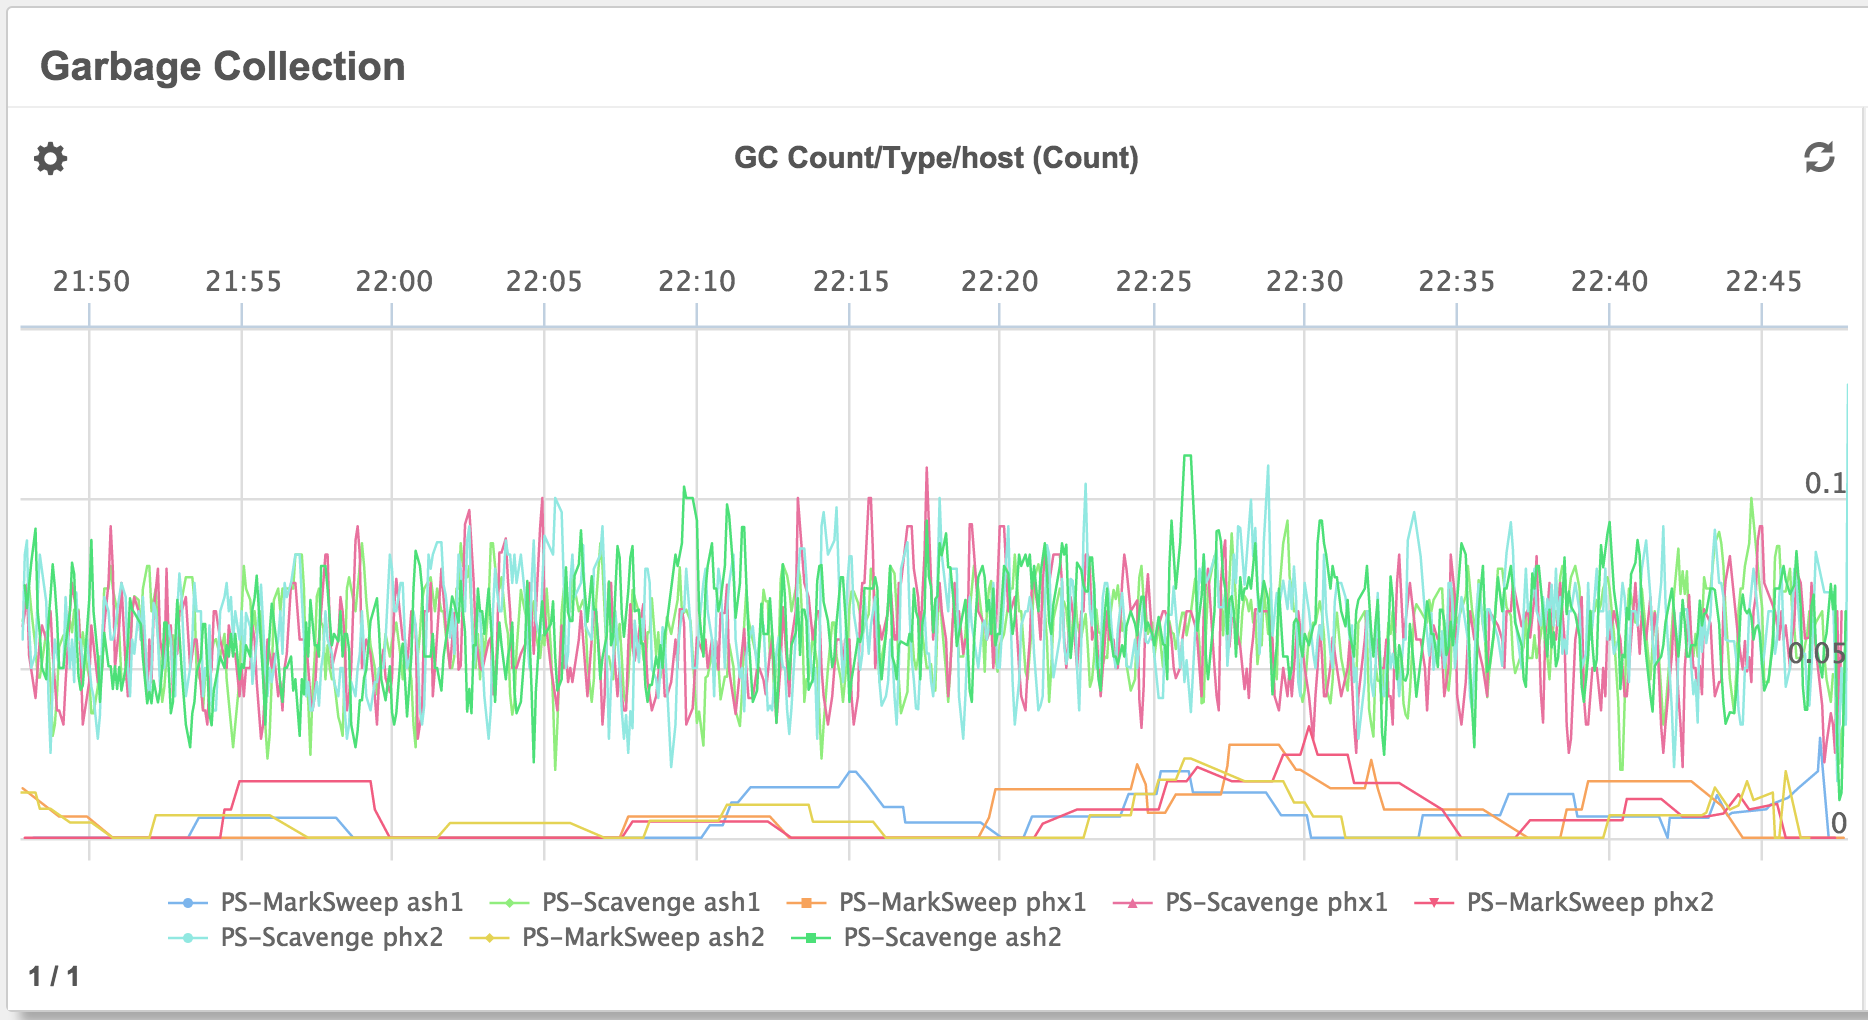
\includegraphics[width=0.8\textwidth]{images/metrilyx.png}
       \caption{Vizualizácia časových rád OpenTSDB pomocou Metrilyx}\cite{Metrilyx}
\end{center}
\end{figure}

\section{InfluxDB}
InfluxDB je platforma v jazyku Go na zbieranie, uchovávanie, vizualizáciu a správu časových dát. InfluxDB je určená na použitie ako úložisko dát v takých prípadoch, ktoré zahŕňajú veľké množstvo
dát označených časovou známkou, vrátane DevOps monitorovania, aplikačných metrík, senzorových dát internetu vecí, a na analýzu dát v reálnom čase.\cite{21} Užívateľ môže vytvoriť viacero nezávislých databáz. 
Dáta sa zapisujú a čítajú pomocou rozhrania príkazového riadka, rôznych klientskych knižníc, alebo pomocou HTTP API. Na vizualizáciu dát používa modul \emph{chronograf}.

\subsection{Politiky udržiavania}
Každá databáza obsahuje pravidlá, ktoré definujú, po akú dobu majú byť ukladané dáta časových rád a koľko kópií dát má byť vytvorených. Jedna databáza môže mať niekoľko takýchto politík. Pri zápise 
do nej je môžné špecifikovať, ktorá politika sa má pre zápis použiť. Pri vytvorení databázy je automaticky vytvorená jedna politika.

\subsection{Kontinuálne dotazovanie a agregácia}
Databáza je schopná periodicky vykonávať požiadavky na dáta. Cieľom je zmenšovanie objemu dát. Ide o zhlukovanie dát s vysokou frekvenciou zberu, čím vzniknú dáta s menšou hustotou zberu. Táto hodnota je 
potom zvyčajne uložená do inej databázy.

\section{RRDTool}
RRDTool je nástroj na uchovávanie, spravovanie a vizuálizáciu časových dát. Využíva round-robin databázu. Je to databáza s dopredu daným maximálnou časovým rozpätím, za ktoré uchováva metrické dáta.
V prípade, že príde požiadavka na zápis hodnoty 
a databáza je už plná, dôjde k prepisu najstaršej hodnoty. Tento nástroj takisto obsahuje funkcie na konsolidáciu dát. Konsolidovaná hodnota je typicky priemer, minimum alebo maximum z viacerých hodnôt zozbieraných 
za dlhší časový úsek. Tieto hodnoty sú taktiež ukladané do round-robin archívu.



\chapter{Metriky}
Každá z technológií cloudového výpočetného strediska je zdrojom mnohých dát o vyťažení zdrojov. Je potrebné určiť, ktoré zdroje monitorovať a ktoré metriky zberať. V prípade MetaCentra podstatné
zdroje predstavujú \emph{procesor, pamät, pevné disky a sieťové rozhrania}. Je vhodné mať také metriky pre všetky využívané cloudové technológie,
ktoré je možné nejakým spôsobom porovnať medzi sebou. V prípade procesora sa jedná o jeho aktuálne vyťaženie, ale zároveň je zaujímavým údajom aj prepočítaný procesorový čas. Táto metrika môže byť efektívnym
nástrojom pre následné učtovanie jednotlivým úžívateľom. Keďže majú ale tieto technológie principiálny rozdiel vo svojom určení, nie je možné vždy o každom zdroji zberať rovnaké dáta. 
O distribuovaných výpočtoch napríklad nie je možné efektívne zistiť aktuálne vyťaženie procesora. Takéto úlohy sa počítajú na viacerých uzloch clustera. O poradí a rozmiestnení požiadaviek na zdroje
rozhodouje riadiaca aplikácia, takže sa nejedná o jeden procesor. Táto aplikácia má ale prehľad o tom, koľko času strávil celý cluster počítaním danej úlohy. Takže v určitom ohľade zrovnateľná s virtuálnym
strojom a jeho spotrebou procesorového času.

Podobná situácia nastáva aj u monitorovania sieťových rozhraní. Distribuované výpočty využívajú sieť svojským spôsobom a len na účel vypočítania komplexnejšieho problému. Jedná sa o prepojenie
uzlov v rámci clustera. Je to jednoúčelová vysokorýchlostná sieť. Z hľadiska poskytovania výpočetných kapacít dáva väčší zmysel orientácia na využívanie konektivity smerom do internetu. 

\subsection{Význam popisných údajov metrík}
Metrické dáta vypovedajú o využití zdrojov. Vieme určiť ako dlhý čas a v akej miere bol využívaný výpočtový výkon. Z nich samotných nevieme presne určiť, kto zdroje využíval. Pre to aby mali tieto dáta zmysel 
pre neskoršie účtovanie, je potrebné mať možnosť ich priradiť k užívateľom, či už sa jedná o vlastnika virtuálneho stroja alebo uživateľa, ktorý spustil kontrétnu úlohu. Na základe týchto ďalších popisných  údajov je potom 
možné zisťovať, kto zdroje vyťažoval za časové obdobie najviac a podľa toho stanoviť prípadnú cenu za používanie zdrojov. Okrem identity je vhodné metriky popisovať aj ďalšími údajmi, ako je miesto, kde
sa zdroj nachádza, názov stroja, ktorý poskytuje svoje kapacity, a ďalšie špecifické údaje, ktoré sa týkajú jednotlivých technológií, ktoré budem popisovať konkrétnejšie v ďalších častiach.

\subsection{Periodicita zberania metrík}
Zberané metriky sa líšia tým, ako veľmi sa v čase menia. Kým záťaž procesora, vstupno-výstupné operácie alebo množstvo prenesených dát sa mení v čase pomerne rýchlo, veľkosť clustera v počte poskytnutých procesorov 
alebo virtuálnej pamäte sa nemení tak často. Má preto zmysel uvažovať o kontrole intervalu zbierania jednotlivých metrík. Nie len na úrovni zhluku metrík pre konrétnu technológiu ale aj pre jednotlivé metriky samostatne.

\subsection{Formát hodnoty metriky}
Metriky ako záznamy obsahujú čas, kedy bola hodnota nameraná, samotnú hodnotu nejakého sledovaného javu a popisné dáta. Na metrické
hodnoty sa môžeme pozerať ako na prírastky alebo ako na absolútne hodnoty. Prírastky hovoria o rozdiele aktuálne nameranej hodnoty 
a poslednej hodnoty. Absolútne hodnoty predstavujú aktuálnu nameranú hodnotu využitia zdroja. 

\section{Docker}
\subsection{Sieť}
Aby mohli medzi sebou jednotlivé kontajnery komunikovať, Docker im poskytuje sieťové rozhrania. Každé rozhranie má nakonfigurovanú sieť,
do ktorej patrí. Na to, aby kontajnery spolu mohli komunikovať, musia byť členmi rovnakej siete. Komunikácia naprieč sieťami nie je možná.
Užívatelia si môžu definovať vlastné siete. Docker na vytvorenie týchto sietí poskytuje dva ovládače.

\subsubsection{Sieť typu most}
Je to jednoduchý typ siete určený pre malé siete. Je ju možné vytvoriť príkazom 
\\
{\em \$ docker network create --driver bridge NÁZOV\_SIETE}
\\ \\
Po vytvorení siete je možné spustiť kontajnery v tejto sieti príkazom
\\ \\
{\em \$ docker run --net=NÁZOV\_SIETE --name=NÁZOV\_KONTAJNERA}

\subsubsection{Prekladaná sieť}
Docker umožňuje vytvoriť aj sieť, v ktorej sa nachádza viacero hosťujúcich počítačov zároveň. To umožňuje komunikovať medzi sebou aj kontajnerom,
ktoré sú spustené v rozličných sieťach, prípadne na inom hosťujúcom počítači.


\subsubsection{Metriky siete}
Pre jednotlivé sieťové rozhrania je možné zbierať tieto metriky:
\begin{description}
\item[rx\_bytes] - počet prijatých bajtov
\item[rx\_dropped] - počet prichádzajúcich zahodených bajtov
\item[rx\_error] - počet chybných bajtov
\item[rx\_packets] - počet prijatých paketov
\item[tx\_bytes] - počet odoslaných bajtov
\item[tx\_dropped] - počet zahodených bajtov pri pokuse o odoslanie
\item[tx\_errors] - počet odoslaných chybných bajtov
\item[tx\_packets] - počet odoslaných paketov
\end{description}

\subsection{Pamäť}
Cez API Dockeru je možné získať nasledovné metriky pamäte.
\begin{description}
\item[usage] - spotreba pamäte
\item[failcnt] - počet chýb
\end{description}
Docker neposkytuje údaj o tom, koľko pamäte poskytuje hosťujúci počítač. Zistiť tento údaj však v implementácií nepredstavuje problém,
a preto je tiež zberaná táto metrika.

\subsection{Procesor}
Procesor predstavuje jeden z najdôležitejších údajov o vyťažení zdrojov. Docker poskytuje viaceré metriky o procesore, ktorých hodnoty 
predstavujú výpočetný čas strávený na procesore: 
\begin{description}
\item[percpu\_usage] - využitie jednotlivých jadier procesora
\item[usage\_in\_usermode] - 
\item[total\_usage] - 
\item[usage\_in\_kernelmode] - 
\item[system\_cpu\_usage] - 
\end{description}

\section{libvirt/KVM}

\subsection{Metriky siete}
Pre jednotlivé sieťové rozhrania je možné zbierať tieto metriky:
\begin{description}
\item[rx\_bytes] - počet prijatých bajtov
\item[rx\_dropped] - počet prichádzajúcich zahodených bajtov
\item[rx\_error] - počet chybných bajtov
\item[rx\_packets] - počet prijatých paketov
\item[tx\_bytes] - počet odoslaných bajtov
\item[tx\_dropped] - počet zahodených bajtov pri pokuse o odoslanie
\item[tx\_errors] - počet odoslaných chybných bajtov
\item[tx\_packets] - počet odoslaných paketov
\end{description}

\subsection{Metriky pamäte}
\begin{description}
\item[VIR\_DOMAIN\_MEMORY\_STAT\_SWAP\_IN] - The total amount of memory written out to swap space (in kB).
\item[VIR\_DOMAIN\_MEMORY\_STAT\_SWAP\_OUT] - Page faults occur when a process makes a valid access to virtual memory that is not available. When servicing the page fault, if disk IO is required, it is considered a major fault. If not, it is a minor fault. These are expressed as the number of faults that have occurred.
\item[VIR\_DOMAIN\_MEMORY\_STAT\_MAJOR\_FAULT] - počet chybných bajtov
\item[VIR\_DOMAIN\_MEMORY\_STAT\_MINOR\_FAULT] - počet prijatých paketov
\item[VIR\_DOMAIN\_MEMORY\_STAT\_UNUSED] - The amount of memory left completely unused by the system. Memory that is available but used for reclaimable caches should NOT be reported as free. This value is expressed in kB.
\item[VIR\_DOMAIN\_MEMORY\_STAT\_AVAILABLE] - The total amount of usable memory as seen by the domain. This value may be less than the amount of memory assigned to the domain if a balloon driver is in use or if the guest OS does not initialize all assigned pages. This value is expressed in kB.
\item[VIR\_DOMAIN\_MEMORY\_STAT\_ACTUAL\_BALLOON] - Current balloon value (in KB).
\item[VIR\_DOMAIN\_MEMORY\_STAT\_RSS] - Resident Set Size of the process running the domain. This value is in kB
\item[VIR\_DOMAIN\_MEMORY\_STAT\_NR] - The number of statistics supported by this version of the interface. To add new statistics, add them to the enum and increase this value.
\end{description}

\subsection{Metriky zápisu dát}
\begin{description}
\item[rd\_req] - number of read requests
\item[rd\_bytes] - number of read bytes
\item[wr\_req] - number of write requests
\item[wr\_bytes] - number of written bytes
\item[errs] - In Xen this returns the mysterious 'oo\_req'.
\end{description}

\subsection{Metriky CPU}
Libivirt poskytuje údaje o tom, koľko výpočetného času strávil daný virtuálny stroj na procesore hosťujúceho počítača. Keďže sa jedná
o plnú hardvérovú vritualizáciu, má zmysel zberať aj informácie o tom, ako sú vyťažené jednotlivé virtuálne procesory.


\section{Hadoop}
\subsection{Cluster Metrics API}
Toto API poskytuje metriky o vyťažení celého clustera.
\begin{description}
\item[appsSubmitted] - The number of applications submitted
\item[appsCompleted] - The number of applications completed
\item[appsPending] - The number of applications pending
\item[appsRunning] - The number of applications running
\item[appsFailed] - The number of applications failed
\item[appsKilled] - The number of applications killed
\item[reservedMB] - The amount of memory reserved in MB
\item[availableMB] - The amount of memory available in MB
\item[allocatedMB] - The amount of memory allocated in MB
\item[totalMB] - The amount of total memory in MB
\item[reservedVirtualCores] - The number of reserved virtual cores
\item[availableVirtualCores] - The number of available virtual cores
\item[allocatedVirtualCores] - The number of allocated virtual cores
\item[totalVirtualCores] - The total number of virtual cores
\item[containersAllocated] - The number of containers allocated
\item[containersReserved] - The number of containers reserved
\item[containersPending] - The number of containers pending
\item[totalNodes] - The total number of nodes
\item[activeNodes] - The number of active nodes
\item[lostNodes] - The number of lost nodes
\item[unhealthyNodes] - The number of unhealthy nodes
\item[decommissionedNodes] - The number of nodes decommissioned
\item[rebootedNodes] - The number of nodes rebooted
\end{description}

\subsection{Cluster Application API}
Tento koncový bod API poskytuje informácie o jednotlivých aplikáciách, ktoré sú spustené na clusteri.
\begin{description}
\item[id] - The application id
\item[user] - The user who started the application
\item[name] - The application name
\item[Application Type] - The application type
\item[queue] - The queue the application was submitted to
\item[state] - The application state according to the ResourceManager - valid values are members of the YarnApplicationState enum: NEW, NEW\_SAVING, SUBMITTED, ACCEPTED, RUNNING, FINISHED, FAILED, KILLED
\item[finalStatus] - The final status of the application if finished - reported by the application itself - valid values are: UNDEFINED, SUCCEEDED, FAILED, KILLED
\item[progress] - The progress of the application as a percent
\item[trackingUI] - Where the tracking url is currently pointing - History (for history server) or ApplicationMaster
\item[trackingUrl] - The web URL that can be used to track the application
\item[diagnostics] - Detailed diagnostics information
\item[clusterId] - The cluster id
\item[startedTime] - The time in which application started (in ms since epoch)
\item[finishedTime] - The time in which the application finished (in ms since epoch)
\item[elapsedTime] - The elapsed time since the application started (in ms)
\item[amContainerLogs] - The URL of the application master container logs
\item[amHostHttpAddress] - The nodes http address of the application master
\item[allocatedMB] - The sum of memory in MB allocated to the application’s running containers
\item[allocatedVCores] - The sum of virtual cores allocated to the application’s running containers
\item[runningContainers] - The number of containers currently running for the application
\item[memorySeconds] - The amount of memory the application has allocated (megabyte-seconds)
\item[vcoreSeconds] - The amount of CPU resources the application has allocated (virtual core-seconds)
\end{description}cit

\subsection{Node Application API}
Toto API poskytuje metriky o využití jednotlivých uzlov clusteri.
\begin{description}
\item[rack] - The rack location of this node
\item[state] - State of the node - valid values are: NEW, RUNNING, UNHEALTHY, DECOMMISSIONED, LOST, REBOOTED
\item[id] - The node id
\item[nodeHostName] - The host name of the node
\item[nodeHTTPAddress] - The nodes HTTP address
\item[healthStatus] - The health status of the node - Healthy or Unhealthy
\item[healthReport] - A detailed health report
\item[lastHealthUpdate] - The last time the node reported its health (in ms since epoch)
\item[usedMemoryMB] - The total amount of memory currently used on the node (in MB)
\item[availMemoryMB] - The total amount of memory currently available on the node (in MB)
\item[usedVirtualCores] - The total number of vCores currently used on the node
\item[availableVirtualCores] - The total number of vCores available on the node
\item[numContainers] - The total number of containers currently running on the node
\end{description}

\chapter{Analýza a návrh}
\section{MetaCentrum}
Projekt MetaCentrum vznikol v roku 1996 a od roku 1999 je jeho činnosť zastrešovaná organizáciou CESNET. Zaoberá sa budovaním nárdonej gridovej infraštruktúry a prepojením s podobnými projektami za hranicami
Českej republiky. Projekt je oficiálnou súčasťou Európskej gridovej iniciatívy (EGI). Úlohou MetaCentra je predovšetkým koordinácia a rozširovanie infraštruktúry či už o vlastné zdroje alebo prostredníctvom
partnerov, ktorý poskytujú výpočetný výkon svojich clusterov. Jedná sa hlavne o akademickú spoluprácu. MetaCentrum spravuje výpočetné prostriedky a dátové úložiská AV, JČU, MU, MZLU, UK, VUT, ZČU.
V súčasnosti disponuje (stav k 30.7. 2010) 1500 jadrami CPU, 100 TB využiteľnej diskovej kapacity v podobe poľa a 400 TB kapacity v podobe pások. Služby využíva 385 registrovaných aktívnych užívateľov, ktorí 
spolu na 750 tisíc úlohách využili 7 miliónov hodín procesorového času.

MetaCentrum primárne poskytuje svoj výpočetný výkon a úložnú kapacitu. Taktiež sprístupňuje svoje programové vybavenie a vývojové prostredie a hlavne množstvo aplikácií využívaných na výskumné účely, ako napr. 
Ansys, Gaussian, Matlab, Mathematica. Taktiež sa venuje vývoju v oblasti gridového a cloudového počítania, napr. v oblasti plánovania, gridového middleware, optimalizácie a paralelizácie výpočtov a virtualizácie
infraštruktúry. Dôležitou funkciou je účasť na medzinárodných projektoch, využívanie medzinárodnej výpočetnej infraštruktúry a využívanie skúseností na rozvoj v domácom prostredí.

\section{Požiadavky na aplikáciu}
\subsection{Vysoký monitorovací výkon}
Cloudová infraštruktúra MetaCentra pozostáva z mnohých výpočetných uzlov. Sú prepojené sieťami s veľkou prenosovou kapacitou a vysokou priepustnosťou. Je potrebné zbierať dáta o využití množstva zapojených
clusterov a uzlov, na ktorých je tiež spustených mnoho výpočetných úloh či virtuálnych strojov. Metriky sú zbierané periodicky v určitých intervaloch z jednotlivých uzlov. Veľká záťaž je kladená na databázu, do ktorej
sú tieto metrické dáta pravidelne odosielané.

\subsection{Nízka nadbytočná záťaž}
Primárnou úlohou cloudu je poskytovanie svojho výpočetného výkonu a prostriedkov. Je žiadúce, aby monitorovacia aplikácia predstavovala čo najmenšiu záťaž pre systémy, na ktorých je spustená. Ak by monitorovanie
samotné spotrebovávalo príliš veľa zdrojov, takto získané metriky by nemali požadovanú presnosť. Je to možné docieliť výberom efektívneho programovacieho jazyka, napr. C, C++, prípadne rýchle skriptovacie 
jazyky ako Python, Ruby či Go. Tie ale predsalen predstavujú istú nadmernú záťaž súvisiacu so spúšťaním interpretera. 
Nie je príliš vhodné používať jazyky, ktoré na svoj beh potrebujú ďalšiu vrstvu v podobe virtuálneho stroja, ako napr. Java.

\subsection{Škálovateľnosť}
Monitorovacia aplikácia by mala poskytovať zrovnateľné výsledky v oblasti rýchlosti odozvy v prípade, že bude spustená na jednom uzle, ale aj v prípade, že jej úlohou bude monitorovať stovky 
výpočetných uzlov s množstvom spustených inštancií, ktoré treba sledovať. To je možné docieliť paralelizovaním dotazov na metriky.

\section{Miesto nasadenia zbernej aplikácie}
Zber metrík je možné realizovať v prípade virtuálnych strojov alebo aplikačných kontajnerov aj z ich vnútra. Bolo by možné v každej
takejto virtualizovanej inštancií spustiť jednoduchú monitorovaciu aplikáciu, ktorá by interagovala priamo so systémom a potom by odosielala dáta.
To ale nie je vhodné riešenie, nakoľko sa nedá predpokladať virtualizovaný operačný systém a zároveň to predstavuje zásah do užívateľského
priestoru. Je lepšie realizovať zber metrík na základe integrácií s aplikáciami, kedy je monitorvacia aplikácia nasadená na fyzickom
operačnom systéme a zberá metriky o virtualizačných aplikáciách, ktoré sú využívané.


\section{Návrh aplikácie}
Monitorovacia aplikácia bude využívať viacero súčastí, ktoré zabezpečujú jednotlivé činnosti súvisiace s monitorovaním tak, ako som ich rozoberal v časi 2.1 Všeobecné problémy monitorovania.
Aplikácia bude zberať metriky, ktoré sú popísané v predošlej kapitole. Samotný proces zberu metrických dát bude zabezpečený aplikáciou collectd. Oproti ostatným dostupným aplikáciám disponuje
veľkou mierou rozšíriteľnosti, kde je možné rozširovať nie len škálu dát, ktoré sa majú zberať, ale aj spôsobom, ako a kam sa budú dané dáta zapisovať. Ďalej umožňuje rozšíriť funkcionalitu
aj v systéme upozornení. Collectd bude zabezpečovať prípadné odosielanie notifikácií prostredníctvom emailu. Ďalšou z výhod zvolenej aplikácie je, že na uskutočňovanie zberu a zápisu používa viacero
paralelne bežiacich vlákien, ktoré si medzi sebou rovnomerne delia záťaž. Ich počet je možné definovať pri konfigurácií. 
\\Jednou z ďalších výhod collectd oproti iným softvérom je spôsob, akým pristupuje k spúšťaniu kontrol. Podľa konfigurácie pri štarte zistí, ktoré moduly sa budú používať. Takisto dôjde ku konfigurácií 
jednotlivých modulov, napr. nastavenie potrebných ciest k požadovaným súborom. Následne dôjde k inicializácií jednotlivých modulov. V tejto fáze moduly inicializujú prostriedky, ktoré potrebujú v priebehu 
zberu metrík. Napr. pripojenie na správcu kontajnerov alebo hypervízora. Nie je efektívne, aby boli tieto prostriedky incializované pri
každej požiadavke na metriku, pretože by to spomaľovalo proces samotného zberu dát. Takýto spôsob bol jedinou možnosťou pri niektorých iných aplikáciách.
\\Potom nasleduje fáza behu. Collectd beží v režime démona na pozadí a periodicky spúšťa jednotlivé moduly, ktoré zisťujú metrické dáta. 
V rámci modulov sa periodicky zisťuje, ktoré virtuálne stroje alebo kontajnery sú spustené a ktorých sa tým pádom budú zberať metriky. 
\\Po nameraní hodnoty collectd inicializuje zápis prostredníctvom modulu Write TSDB. Tu dochádza k ďalším optimalizáciám, ako sú cachovanie
hodnôt a ich odosielanie vo väčších dávkach.
\\V prípade, že je potrebné démona ukončiť, dôjde najprv k ukončeniu jednotlivých modulov. Až v tejto fáze moduly uvoľnia všetky prostriedky, ktoré mali naalokované.
\\Samotný collectd bez pluginov predstavuje riadiaciu aplikáciu v podobe démona, ktorá na svoju inštaláciu vyžaduje minimum závislostí. To je ďalšou z výhod, keďže 
démon na zber metrík bude nainštalovaný na každom monitorovanom uzle.
\\Na zápis monitorovacích dát bude využitá databáza časových rád OpenTSDB. Budem sa jej venovať v nasledujúcej časti.
\\Takýto návrh zabezpečuje decentralizované a škálovateľné riešenie, kedy je distribuovaný nielen zber metrických údajov, ale aj ich zápis a uchovávanie.

\subsection{Centrálny systém notifikácií a manažmentu zberných modulov}
Vyššie popísané riešenie predstavuje decentralizovanú architektúru. Každá zo sond funguje nezávisle, čo sťažuje prípadné mechanizmy konfigurácie
a riešenie krízových situácií ako napr. zastavenie činnosti démona. Toto je jeden z aspektov kde má navrch napr. systém Zabbix. Súčasťou
môjho riešenia bude zároveň aplikácia, ktorá bude spravovať konfigurácie jednotlivých inštancií collectd, umožní ich meniť a podľa toho ich reštartovať.
Umožní prehliadať notifikácie z jednotlivých sond a manuálne ovládať inštancie a ich moduly. To bude zároveň vyžadovať modifikáciu démona
collectd, ktorý v súčasnosti neumožňuje reštartovanie jednotlivých modulov.

\section{OpenTSDB}
Ako databázu na uchovávanie časových dát som si zvolil OpenTSDB. Dôvodom je používanie databázy HBase. Je to distribuovaná databáza určená pre veľké objemy dát v rádoch stoviek miliónov a milárd záznamov. 
Je typom NoSQL databázy. Oproti SQL databázam je linárne škálovateľná. Ak dôdje k zdvojnásobeniu výpočetných zdrojov, dôjde aj k zdvojnásobeniu výkonu databázy. To je dôležité pri zbere časových dát z mnohých
uzlov, ktoré sa v infraštruktúre MetaCentra nachádzajú. Ďalším dôvodom je, že v MetaCentre je aktuálne databáza HBase využívaná, čo predstavuje zjednodušenie nasadenia. 


\chapter{Implementácia}
Využijem existujúcu aplikáciu na zbieranie metrických dát \emph{collectd}. Tá poskytuje mechanizmy na periodické spúšťanie merania metrík,
analýzu zozbieraných hodnôt a generovanie hlásení. Na zbieranie jednotlivých metrík som vytvoril moduly pre tento program. Tieto údaje následne bude odosielať do databázy OpenTSDB
pomocou modulu WriteTSDB.

\section{Techniky zbierania metrík}

\subsection{Docker}
Na komunikáciu s Dockerom je možné využiť:
\begin{description}
\item[príkazy aplikácie v príkazovom riadku]
\item[Remote API]
\end{description}

Používanie príkazov aplikácie môže byť o čosi rýchlejšie, ale následne by bolo potrebné analyzovať textový výstup programu.
Rozhodol som sa použiť Remote API. Toto API funguje pre účely monitorovania na princípe REST a odpovede vracia vo formáte JSON, čo predstavuje zjednodušenie spracovania výstupu. Démon Dockeru "počúva" na 
lokálnom sockete, čo by nemalo spôsobovať výrazné oneskorenie odpovede. Každému kontajneru zodpovedá adresa, ktorá zahŕňa identifikačný reťazec kontajnera.

\subsection{libvirt/KVM}
Na získavanie metrických údajov o virtuálnych strojoch som použil knižnicu libvirt. Je to knižnica napísaná v jazyku C. Poskytuje množstvo
rozhraní, ktoré umožňujú vytvárať virtuálne stroje, zapínať ich a vypínať, meniť ich konfiguráciu. Poskytuje tiež údaje o tom, ako virtuálny
stroj využíva virtualizované zdroje. 
\\Najprv je potrebné vytvoriť spojenie s hosťujúcim počítačom. Toto je udržované počas celého zberu metrík. Cez vytvorené spojenie
je možné zisťovať, ktoré virtuálne stroje sú spustené. V periodických intervaloch aktualizujem zoznam bežiacich strojov a odosielam
metriky len o nich.
\\Collectd už obsahoval plugin pre libvirt, no bolo potrebné doplniť niektoré popisné údaje metrík, ako názov hosťujúceho počítača,
názov virtuálneho stroja a iné.

\subsection{Hadoop}
Na monitorovanie Hadoopu som si zvolil REST API YARN-u. YARN zabezpečuje správu zdrojov a plánovanie/monitorovanie vykonávania úloh do dvoch
oddelených démonov.\cite{23} ResourceManager je autoritou, ktorá rozhoduje o využívaní zdrojov aplikáciami v celom systéme. NodeManager
je agent, nainštalovaný na jednotlivých uzloch, ktorý sa stará o beh kontajner a monitorovanie zdrojov, ktoré spotrebovávajú. Toto
nahlasuje ResourceManagerovi. Preto som zvolil toto API.
\\REST API poskytuje odpovede vo formáte JSON a XML. Vo svojej implementácií využívam odpovede vo formáte JSON.

\section{libcurl}
libcurl je voľne šíriteľná klientska knižnica v jazyku C určená na manipuláciu so zdrojmi identifikovanými pomocou URL. Podporuje
množstvo protokolov ako FTP, FILE, HTTPS, IMAPS, LDAP, POP3, SMTP, SCP atď. Podpourje taktiež SSL certifikáty,
HTTP POST a PUT metódy a rôzne formy autentifikácie. V mojej implementácií túto knižnicu využívam na získavanie metrík zo systému
Hadoop. Využívané REST API sú chránené autentifikačným mechanizmom Kerberos. libcurl vie využiť autorizačné tokeny,
ktoré sú vygenerované pri autentifikácií pomocou Kerberosu. Posiela ich spolu s HTTP GET žiadosťou a týmto spôsobom
sa autentifikuje voči Hadoopu.
\\libcurl je ľahko prenositeľná medzi rôznymi platformami, ako sú Solaris, BSD platformy, Windows, Linux, OS X a iné. Je vláknovo
bezpečná, rýchla, dobre zdokumentovaná a kompatibilná s protokolom IPv6. \cite{24}

\section{libpthread}
libpthread je knižnica, ktorá umožňuje programovanie aplikácií s paralelne vykonávanými procedúrami. Tie sa nazývajú vlákna. Paralelizáciu
v systéme na vyššej úrovni prináša koncept procesov. Pri
vytváraní procesu ale dochádza k režijnej záťaži v operačnom systéme. Procesy si v systéme udržujú viacero parametrov, ako identifikačné
číslo, identifikáciu užívateľa, premenné prostredia, zásobník, haldu, registre, zdieľané knižnice a reagujú na signály. Vlákna využívajú
tieto atribúty a zavádzajú menšiu množinu parametrov a kontrolných signálov, ktoré umožňujú paralelné vykonávanie aj v rámci jedného procesu.
\\Túto knižnicu využívam v plugine pre Docker. V pravidelných intervaloch dochádza k zisťovaniu, ktoré kontajnery sú spustené a na REST API
zodpovedajúcich kontajnerov sú potom paralelne vytvorené a zaslané požiadavky na metrické údaje.

\section{cJSON}
cJSON je miniatúrna knižnica v jazyku C, ktorej úlohou je prevod reťazca vo formáte JSON do hierarchickej štruktúry objektov. Zjednodušuje
to analýzu obdržaných informácií vo formáte JSON. Keďže jazyk C nepozná
objekty, namiesto toho sú používané štruktúry jazyka C. Knižnica neobsahuje žiadne závislosti, na jej činnosť sú potrebné dva súbory - 
jeden so zdrojovými kódmi a jeden hlavičkový súbor.
\\Knižnicu bolo potrebné mierne upraviť, pretože nesprávne narábala s dátovým typom long, ktorý sa vyskytuje ako hodnota niektorých parametrov
vo vracaných JSON reťazcoch. Aj keď knižnica obsahovala tento nedsotatok, zvolil som si ju pre jej minimalistickú formu.

\section{Zapisovací plugin Write TSDB}
Plugin pre collectd s názvom Write TSDB zapisuje metriky do OpenTSDB.\cite{13} Je napísaný v jazyku C. Bolo potrebné ho upraviť,
aby požadovaným spôsobom generoval názvy metrík z údajov, ktoré mu predávajú pluginy zberajúce metriky. Plugin využíva mechanizmy
dočasného zhlukovania správ a ich odosielania vo väčších dávkach. Je možné nakonfigurovať adresu a port, na ktorom je spustený
démon OpenTSDB. Taktiež je možné nakonfigurovať tagy špecifické pre uzol. Toto vo svojej implementácií nevyužívam,
všetky tagy metrík sú generované pluginmi.

\chapter{Záver}

\addcontentsline{toc}{chapter}{Literatúra}
\bibliographystyle{unsrt}
\nocite{*}
\bibliography{dip-lezdik}


\begin{appendix}
\chapter{Kapitola priloha}
\end{appendix}

\end{document}
